L'obbietivo e l'ambizione del mio progetto di tesi è quello di consentire a utenti e aziende di creare la propria piattaforma di E-Learning.
La scelta del progetto è stata dettata dal crescente interesse nei confronti di tali piattaforme negli ultimi anni.
Oggi giorno è facile confondere sistemi di e-learning con i MOOC (Massive Open Online Course), la differenza sostanzizale sta nel fatto che quest'ultimi sono corsi aperti a chiunque,la partecipazione è gratuita e permettono interattività tra gli studenti.
Il primo MOOC nasce intorno al 2007, grazie al lavoro del Professor O’Donnell, dell'Università della Pennsylvania.
L'enorme potenziale di tali sistemi è stata compreso sin da subito e ha portato alla nascita di diverse piattaforme come Coursera, EdX, Udacity.
La Maggior parte di queste offrono corsi organizzati direttamente dagli atenei tra cui troviamo nomi prestigiosi come Stanford, Harvard, Berkeley, MIT. In generale i corsi ricoprono diverse tematiche e vengono erogati direttamente dai Professori degli atenei universitari.
Tutti i corsi sono gratuiti cavalcando la filosofia tipica dei MOOC, viene pero richiesto un compenso nel caso in cui si desidera ottenere una certificazione, rilasciata solo dopo aver superato test per verificare il reale livello di apprendimento.

\begin{figure}[htb] %  figure placement: here, top, bottom
 \centering
 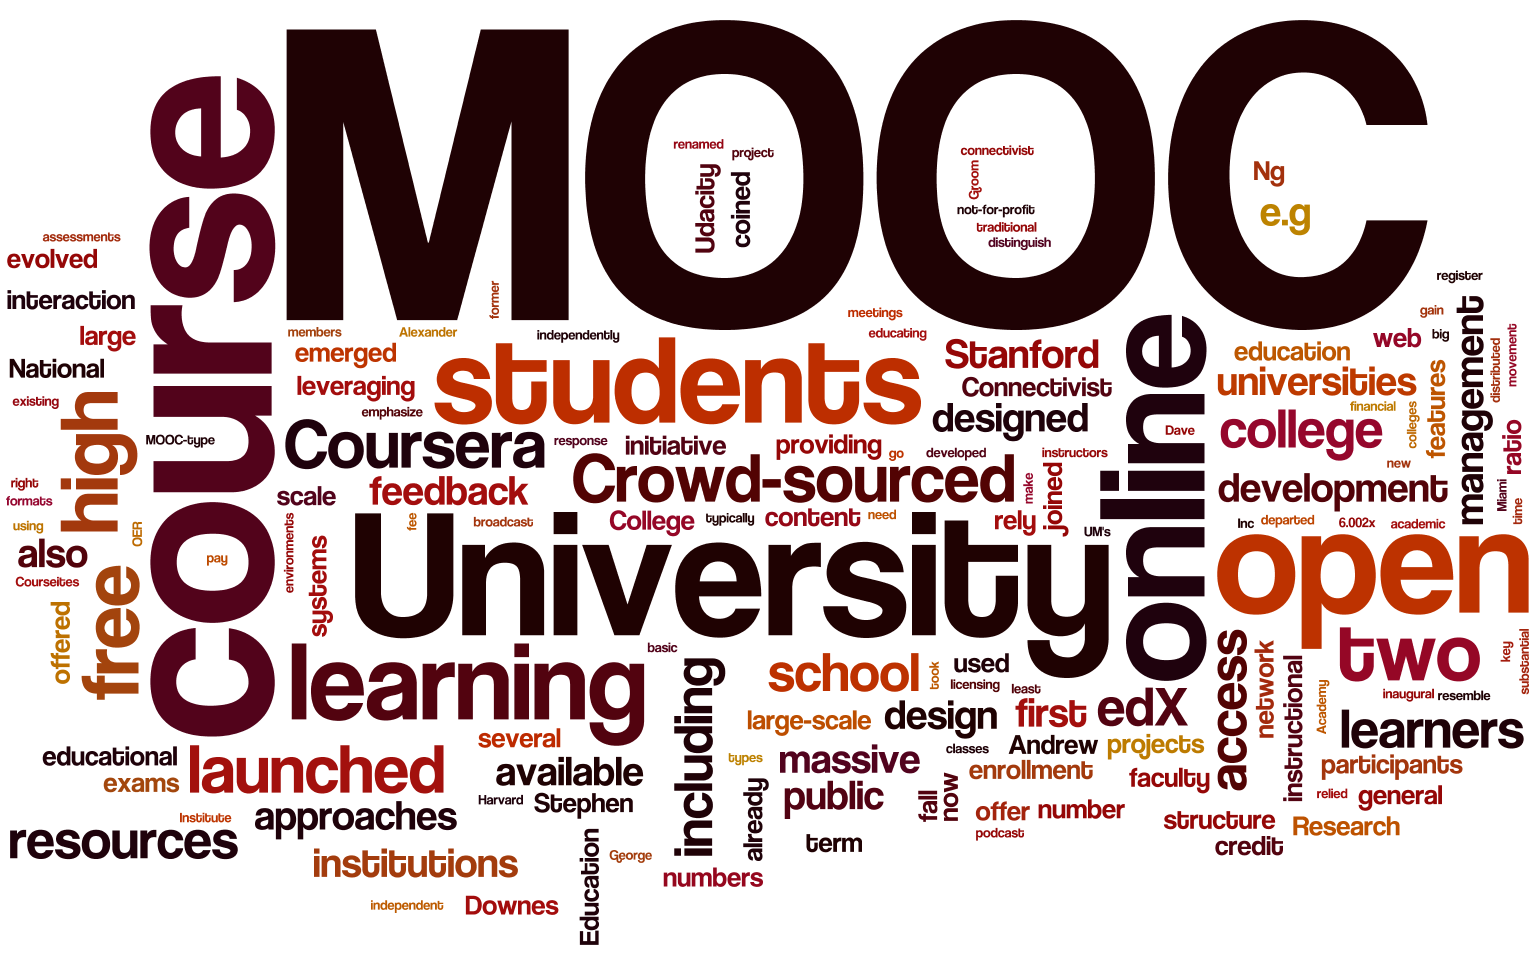
\includegraphics[width=0.8\linewidth]{images/introduction/mooc.png}\hfill
 \caption[Mooc image]{Mooc image}
 \label{fig:fourV}
\end{figure}

Questi sistemi sono stati accolti come una vera e propria rivoluzione nel mondo dell'istruzione, rendendo la formazione accessibile a chiunque eliminando barriere temporali e spaziali. Infatti la comodità e il vantaggio di queste piattaforme è poter seguire corsi universitari a migliaia di chilometri di distanza comodamente da casa e in qualsiasi momento e orario della giornata.

Nelle prime piattaforme di MOOC i corsi erano quindi tenuti dagli stessi docenti degli atenei, questo trend è pero cambiato negli ultimi anni e ha visto la nascita di nuove piattaforme in cui chiunque può creare un proprio corso.

Questa nuova opportunità offerta per esempio dal noto serivzio MOOC di Udemy, ha riscontrato subito un grande successo ed è stata sfruttata da molte persone che ne hanno fatto una vera e propria fonte di guadagno. 

Il mio progetto è invece indirizzato a tutti gli utenti privati, aziende, scuole che vogliono creare una propria piattaforma dove vengono offerti esclusivamente i loro corsi.

Creare un serizio di e-learning richiede investimenti importanti per coprire i costi di realizzazione, storage e traffico dati per lo streaming dei contenuti video.

Già di per se tali costi potrebbero scoragiare un utente medio, inoltre la realizzazione richiede conoscenze tecniche, per la gestione dei video ma anche per lo streaming.
Infatti nonostante HTML5 la gestione video è molto insidiosa, non esiste un standard per lo streaming e inoltre bisogna garantire la fruzione dei contenuti su diversi dispositivi.

Quest'ultimo ostacolo potrebbe essere risolto tramite l'utilizzo di HLS(HTTP Live Streaming) protocollo di comunicazione concepito da Apple e basato su HTTP, che separa il flusso video in chunk e adatta la qualità video sulla base del dispositivo e della connessione.

Infine un ultimo ostacolo potrebbe essere la creazione di una CDN per diminuire i tempi di latenza e garantire la fruzione su larga scala.

%%%%rivedi
Il lavoro di tesi svolto presso il CVDLAB ha come obbietivo finale di supportare l'utente nella realizzazione di una propria piattaforma, progetto ambizioso che richiede ancora tempo, in ogni modo i componenti realizzati durante il mio lavoro sono poi stati riutilizzati nella fase finale per creare un caso d'uso reale: X-learning.


In tale piattaforma di E-learning avremo quindi due ruoli ben distinti: 
\begin{itemize}
\item Admin che puo inserire i corsi e invitare i collaboratori nella propria piattaforma,
\item Utente può navigare la piattaforma e seguire i corsi desiderati
\end{itemize}
Il passo successivo come vedremo nel capitolo dei sviluppi futuri sarà proprio il deploy del servizio per renderlo utilizzabile a chiunque.

%%%%%

% Il mio contributo finale che rappresenta il core di tale progetto è stato la creazione di una piattaforma di E-learning come Udemy dove ogni utente può creare i propri corsi, il passo successivo sara poi come vedremo nel capitolo dei sviluppi futuri il deploy del mio servizio.

La mia tesi è stata divisa in due parti ognuna composta da 3 capitoli.
Nel primo capitolo viene offerta una panoramica sulle piattaforme MOOC esistenti.
Il secondo capitolo è invece una panoramica sui servizi utilizzati per la realizzazione della piattaforma e un analisi dei costi.
Nel terzo capitolo invece vengono descritte le tecnologie utilizzate per lo sviluppo.
Con l'inizio della seconda parte della tesi entriamo nel dettaglio del progetto, in particolar modo nel quarto capitolo avremo una panoramica della struttura.
Nel quinto capitolo ci focalizzeremo sui componenti principali che ho realizzato nel progetto e descrivero come sono stati realizzati.
Nel sesto e ultimo capitolo ci sarà una breve conclusione e i possibili sviluppi futuri.
